\chapter{双耳渲染算法 }

本章对三种典型的双耳渲染算法的原理进行详细介绍,主要包括虚拟听觉重放技术、基于~Ambisonics~的虚拟扬声器方法和基于球谐分解的双耳渲染算法,其中基于球谐分解的双耳渲染算法是本文的研究重点。并给出了双耳渲染中至关重要的头相关传递函数、球谐函数的定义及性质,以及球傅里叶变换及其逆变换等基础知识,为后续工作奠定理论基础。

\section{虚拟听觉重放技术}


人类是通过双耳进行声音感知的,除了可以感知声音的响度、音调和音色,还可以对声源的方位和距离进行判断。声源发出的声音经过头部、躯干、耳廓等散射和反射后到达双耳,因此双耳信号中包含了大多数声源定位的因素,例如双耳时间差和双耳声级差。虚拟听觉方法是指采用信号处理的方法来模拟声波经由头部、躯干、耳廓等人体生理结构的散射和反射的过程。声波从声源到双耳的传输过程可以看作一综合滤波器,该滤波器可以通过头相关脉冲响应(HRIR)和头相关传递函数(HRTF)来描述。


\subsection{头相关传递函数~HRTF}
头相关传递函数(Head-related~Transfer~Function~,~HRTF)定义为自由场情况下从声源到双耳的频域传输函数,表达了生理结构对声波的综合滤波效果\tcite{book_xiebosun}。
如式~\eqref{hrtf_definition}~所示,HRTF~是声源到头中心距离~$r$、声源的方位角~$\theta$、 仰角~$\phi$、 频率~$f$~和人头半径~$a$~的函数。
当声源位于远场时,HRTF~与距离无关,一般略去参数~$r$。
\begin{equation}
\begin{split}
H_{\text{L}} = H_{\text{L}}(r,\theta,\phi,f,a)=\frac{P_{\text{L}}(r,\theta,\phi,f,a)}{P_{0}(r,f)}~, \\
H_{\text{R}} = H_{\text{R}}(r,\theta,\phi,f,a)=\frac{P_{\text{R}}(r,\theta,\phi,f,a)}{P_{0}(r,f)}~,
\end{split}
\label{hrtf_definition}
\end{equation}
式中:$P_{0}$~是头移开后点声源在头中心位置处的频域复数声压,$P_{\text{L}}$、$P_{\text{R}}$~分别为左右耳的频域复数声压。
每个人的生理结构和尺寸不同,式~\eqref{hrtf_definition}~中参数~$a$~的引入就是为了体现~HRTF~的个性化特征,一般不涉及个性化~HRTF~时略去参数~$a$。

严格来说,$P_{\text{L}}$、$P_{\text{R}}$~应定义为左、右耳鼓膜处的电压。但实际测量表明,至少在~14~kHz~ 以下的频率,整个耳道可以近似为一维传输。
所以耳道入口、鼓膜,甚至耳道内任一点的声压,都可以作为~HRTF~定义中的左、右耳声压~$P_{\text{L}}$~、$P_{\text{R}}$~,它们都包含了有关声源空间位置的信息,并且不同测量点的声压之间可以互相转换。
将耳道声压的测量点称为参考点,耳道内任意参考点的声压统称为双耳声压。

在时域上,HRTF~表示为头相关脉冲响应(Head-related~Impulse~Response~,~HRIR),HRIR~和~HRTF~是一对傅里叶变换,HRIR~表示声源到双耳的脉冲响应,是声源位置~$r$、$\theta$、$\phi$~和时间~$t$~的函数。HRIR~和~HRTF~包含了众多主要的声源定位因素,但并不是包含全部的定位因素,至少没有包括头部微小转动所产生的动态因素。

\subsection{基于~HRIR~和~BRIR~的虚拟听觉方法}
为了在双耳渲染中产生空间音频效果,我们可以通过将单声道信号与虚拟声源位置对应的~HRIR~卷积来生成虚拟音效。
该技术中双耳声信号和相应的空间信息都是通过信号处理的方法人为产生或虚拟出来的,其中不同的声源信号和方位都是已知的。

在自由场情况下,位置~$(r,\theta,\phi)$~的声源在双耳处产生的声压可以通过相应角度的头相关传递函数~$H_{\text{L}}(r,\theta,\phi,f)$~和~$H_{\text{R}}(r,\theta,\phi,f)$~ 描述。
通过实验测量或理论计算得到头相关传递函数后,将频域信号~$E_{0}(f)$~代入式~\eqref{eq.convtobinaural}~即可计算出双耳声压。
\begin{equation}\label{eq.convtobinaural}
\begin{split}
B_{\text{L}}(f) = E_{0}(f)H_{\text{L}}(r,\theta,\phi,f)\\
B_{\text{R}}(f) = E_{0}(f)H_{\text{R}}(r,\theta,\phi,f).
\end{split}
\end{equation}

然而人耳听音的环境大多都是多声源和混响环境,实际系统中通常需要引入多个声源的叠加,并且需要考虑房间的声学特性,如早期反射和晚期混响。使用~HRIR~进行双耳渲染时,需要先对采集信号进行方位估计和声源分离,再对其进行渲染,如图~\ref{fig:BRS}所示。此时计算量取决于听觉场景的复杂度,场景中声源数目越多,计算量越大。

\begin{figure}[H]
\centering
\includegraphics[width=0.6\textwidth]{figure/chapter2/rendering_based_HRIR_BRIR}
\caption{基于~HRIR~和~BRIR~的方法}
\label{fig:BRS}
\end{figure}

一个概念上简单的例子是通过双耳房间冲激响应(Binaural Room Impulse Response , BRIR)进行渲染。在一个经过声学优化的混响环境下的听音室中,使用放置在某一固定位置的高性能扬声器播放声源信号,并通过放置在理想收听位置的假人头模型,测量扬声器到麦克风的冲激响应即可获取~BRIR。~BRIR~描述了声音从房间里的一点传到听者耳朵的特征,需单独考虑直达波、早期反射、晚期混响,能够准确地捕捉房间的特征,直接对整个环境进行渲染 。使用~BRIR~进行渲染是一种有效的方式来给听者提供身临其境的三维空间音频场景。


假设~$S$~个信号源的空间位置~$(r_{s},\theta_{s},\phi_{s})$~和激励信号~$E_{s}(f)$~已知,通过卷积对应的双耳房间冲激响应获取双耳信号:
\begin{equation}
\begin{split}
B_{\text{L}}(f) = \sum_{s=1}^{S} E_{s}(f)BRIR_{\text{L}}(r_{s},\theta_{s},\phi_{s},f)\\
B_{\text{R}}(f) = \sum_{s=1}^{S} E_{s}(f)BRIR_{\text{R}}(r_{s},\theta_{s},\phi_{s},f),
\end{split}
\end{equation}
其中,$BRIR_{\text{L}}(r_{s},\theta_{s},\phi_{s},f)$~和~$BRIR_{\text{R}}(r_{s},\theta_{s},\phi_{s},f)$~分别声源方位为~$(r_{s},\theta_{s},\phi_{s})$~对应的左耳和右耳的房间冲激响应。


基于~HRIR~和~BRIR~的方法在使用耳机进行回放的过程中,需要根据听者和声源的相对位置选择对应的~HRIR/BRIR~数据(当声源位置未包含在数据库时还需进行插值),再对于每个声源,将源信号与其对应的~HRIR/BRIR~进行卷积的结果求和并反馈给耳机。
当听者处于运动状态时需要快速产生符合真实听感的声像轨迹,除非使用高速、低延时的算法,否则~HRTF~插值和卷积的组合过程可能导致对头部移动的响应产生不可接受的延时。


\section{基于~Ambisonics~的虚拟扬声器方法}\label{section_Ambisonic_virtual_loudspeaker}

对于许多应用,我们希望能够直接对捕获的整个声场进行渲染,而不需要事先知道源的数量或位置,或声学环境的结构。基于~Ambisonics~的虚拟扬声器方法就是其中一种。

首先对~Ambisonics~技术进行简单介绍,该技术是一种基于空间声场球谐函数分解和重构的声音回放技术,其核心思想是使用某一场景中的麦克风阵列(例如,声场麦克风,球形麦克风阵列)捕获来自不同方向的声压波,并通过位于听众周围的扬声器阵列进行重现~\tcite{review_headphone_spatial}。

Ambisonics~技术包括编码和解码两大模块,编码是对声场采集信号进行分解,求得各阶球谐分量;解码则是根据扬声器的位置对各阶分量进行组合得到扬声器激励信号,实现声场重建。
Ambisonics~系统最大的优点在于其编码和解码模块是互相独立的,编码时无需事先知道扬声器的摆放位置,解码时根据扬声器位置选择不同的解码矩阵即可,并且扬声器阵列的摆放具有较高的灵活性,便于实现。

Ambisonics~系统的编解码是在以下假设下进行的:(1)~录制采样的声源为空间某方向入射的平面波;(2)~回放过程中,扬声器发出的声波相对听音位置也可视为平面波。以上假设在声源和扬声器均位于远场时成立\tcite{Ambisonics_yuanchang}。


\subsection{Ambisonics~编码}

对于~Ambisonics~来说,其编码时通过完备正交集球谐函数进行的,通过使用球傅里叶变换对声场进行球谐分解,从而获取声场的球谐系数,接下来将详细介绍。

球谐函数有复数和实数两种等价定义形式~\tcite{williams_fourier_2000}\tcite{2013Hilbert}\tcite{rafaely_fundamentals_2019},其中~$n$~阶~$m$~次复数形式的归一化球谐函数定义如下:
\begin{equation}\label{qiuxiefushu}
Y_{n}^{m}(\theta,\phi) = \sqrt{\frac{2n+1}{4\pi}\frac{(n-m)!}{(n+m)!}}P_{n}^{m}(\cos\theta)e^{im\phi},
\end{equation}
其中,$n=0,1,2,\cdots,~m=0,\pm1,\pm2,\cdots,\pm~n$,$i=\sqrt{-1}$,$(\cdot)!$~表示阶乘,$P_{n}^{m}(\cdot)$~表示关联勒让德函数。
$\sqrt{\frac{2n+1}{4\pi}\frac{(n-m)!}{(n+m)!}}$~是归一化系数,其值由关联勒让德函数决定。~$\theta$~表示俯仰角,定义为方向矢量与~$z$~正轴的夹角,$\phi$~表示水平面的方位角,且~$0^{\circ}\le\theta\le180^{\circ}$~,~$0^{\circ}\le\phi\le360^{\circ}$,角度定义如图~\ref{fig:harmonics_theta_phi_definition}~所示。


\begin{figure}[H]
\centering
\includegraphics[width=0.7\textwidth]{figure/chapter2/harmonics_theta_phi_definition.eps}
\caption{球谐函数角度定义图}
\label{fig:harmonics_theta_phi_definition}
\end{figure}

球谐函数有许多特性,其中最重要的是正交完备性,将在本文中多次应用。不同阶的~$Y_{n}^{m}(\theta,\phi)$~满足以下正交关系式:
\begin{equation}\label{eq.orth}
\int_{0}^{2\pi}\int_{0}^{\pi}[Y_{n}^{m}(\theta,\phi)]^{*}Y_{n^{'}}^{m^{'}}(\theta,\phi)\sin\theta d\theta d\phi = \delta_{nn^{'}}\delta_{mm^{'}},
\end{equation}
式中,$\delta_{nn^{'}}$、$\delta_{mm^{'}}$~为~$\delta$~函数:
\begin{equation}
\delta_{nn^{'}}=\left\{
             \begin{array}{lr}
             1 ,& n=n^{'},  \\
             0 ,& n\neq~n^{'}.
             \end{array}
\right.
\end{equation}

\begin{figure}[H]
\centering
\includegraphics[width=1\textwidth]{figure/chapter2/SH_4order.pdf}
\caption{球谐函数三维图}
\label{fig:SH_4order}
\end{figure}

图~\ref{fig:SH_4order}~为球谐函数的三维图,其中从上到下分别对应~$n=0$~到~$n=4$,从左到右分别对应~$m=-n$~到~$m=n$,当~$m$~取负值时绘制~$Y_n^m$~的虚部,$m$~取实值时绘制~$Y_n^m$~的虚部。图中黄色部分表示正值,绿色部分表示负值。
% 从图中可以看出不同~$n$~和~$m$~下的球谐函数之间正交。


正是因为球谐函数的正交完备性,在很多应用中采用球谐函数作为基底函数,以保证声场的正交分解。如式~\eqref{eq.coe}~所示,声场中任意一点的声压可以看作不同阶球谐函数的叠加:
\begin{equation}\label{eq.coe}
   S(r,\theta,\phi,f)=\sum _{n=0}^\infty \sum _{m=-n}^n S_n ^m(r,f)Y_n ^m(\theta,\phi),
\end{equation}
其中,球谐系数~$S_n ^m(r,f)$~可通过式~\eqref{eq.SFT}~得到。
\begin{equation}\label{eq.SFT}
   S_n ^m(r,f)=\int_{0}^{2\pi}\int _{0}^{\pi}S(r,\theta,\phi,f)[{Y_n^{m}(\theta,\phi)}]^{*}\sin \theta d\theta d\phi.
\end{equation}

式~\eqref{eq.SFT}~称为~$S(r,\theta,\phi,f)$~的球傅里叶变换(Spherical Fourier Transform,SFT),式~\eqref{eq.coe}~称为~$S_n ^m(r,f)$~的反球傅里叶变换(Inverse Spherical Fourier Transform,ISFT),二者构成逆变换。

如式~\eqref{eq.coe}~可知,声场可以看作是无穷个球谐函数的线性组合,然而在实际系统中这是不可实现的,不能实现声场的无限阶球谐分解,需要对原始声场的分解做截断处理,即使用有限阶的球谐函数来对声场进行近似:
\begin{equation}\label{eq.coe_N}
   \hat{S}(r,\theta,\phi,f)=\sum _{n=0}^{N} \sum _{m=-n}^n S_n ^m(r,f)Y_n ^m(\theta,\phi),
\end{equation}
其中,$\hat{S}(r,\theta,\phi,f)$~是~$S(r,\theta,\phi,f)$~的近似值,$N$~是球谐函数阶数的最大值。



这种截断处理必然会影响声场的精度,定义归一化截断误差如下~\tcite{Ward2001Reproduction}:
\begin{equation}\label{eq.varepsilon}
  \varepsilon _N(kr)= \frac{\int_{0}^{2\pi}\int _{0}^{\pi} |S(r,\theta,\phi,f)-\hat{S}(r,\theta,\phi,f)|^2 \sin \theta d\theta d\phi }
  {\int_{0}^{2\pi}\int _{0}^{\pi} |S(r,\theta,\phi,f)|^2 \sin \theta d\theta d\phi } ,
\end{equation}
式中,波数~$k=2\pi f/c$,声速~$c=343~\mathrm{m}/\mathrm{s}$。

对于内部域问题,即所有声源均位于所关注的区域外,内部声压场可以表示为~\tcite{williams_fourier_2000}:
\begin{equation}\label{eq.coeS}
   S(r,\theta,\phi,f)=\sum _{n=0}^\infty \sum _{m=-n}^n A_n ^m(f)j_n(kr)Y_n ^m(\theta,\phi),
\end{equation}
其中,~$A_n ^m(f)=S_n ^m(r,f)/{j_n(kr)}$~是与位置无关的球谐系数,$j_n(\cdot)$~为球贝塞尔函数。

自由场环境下,对于来波方位为~($\theta_{s},\phi_{s}$)~的单位幅度平面波来说,式~\eqref{eq.coeS}~及其截断表示为:
\begin{equation}\label{eq.coeS_planewave}
   S(r,\theta,\phi,f)=\sum _{n=0}^\infty \sum _{m=-n}^n 4\pi i^{n} j_n(kr)\left[ Y_n ^m(\theta_{s},\phi_{s}) \right] ^{*} Y_n ^m(\theta,\phi).
\end{equation}
\begin{equation}\label{eq.coeS_planewave_N}
   \hat{S}(r,\theta,\phi,f)=\sum _{n=0}^{N} \sum _{m=-n}^n 4\pi i^{n} j_n(kr)\left[ Y_n ^m(\theta_{s},\phi_{s}) \right] ^{*} Y_n ^m(\theta,\phi).
\end{equation}

将式~\eqref{eq.coeS_planewave}~和式~\eqref{eq.coeS_planewave_N}~代入到式~\eqref{eq.varepsilon},归一化截断误差可表示为:
\begin{equation}\label{varepsilon1}
  \varepsilon _N(kr)=1-\sum _{n=0}^ N(2n+1)(j_n(kr))^2.
\end{equation}

关于~$kr$~的归一化截断误差~$\varepsilon_N(kr)$~与截断阶数~$N$~之间的关系如图~\ref{Fig:N_kR}所示。

\begin{figure}[H]
\centering
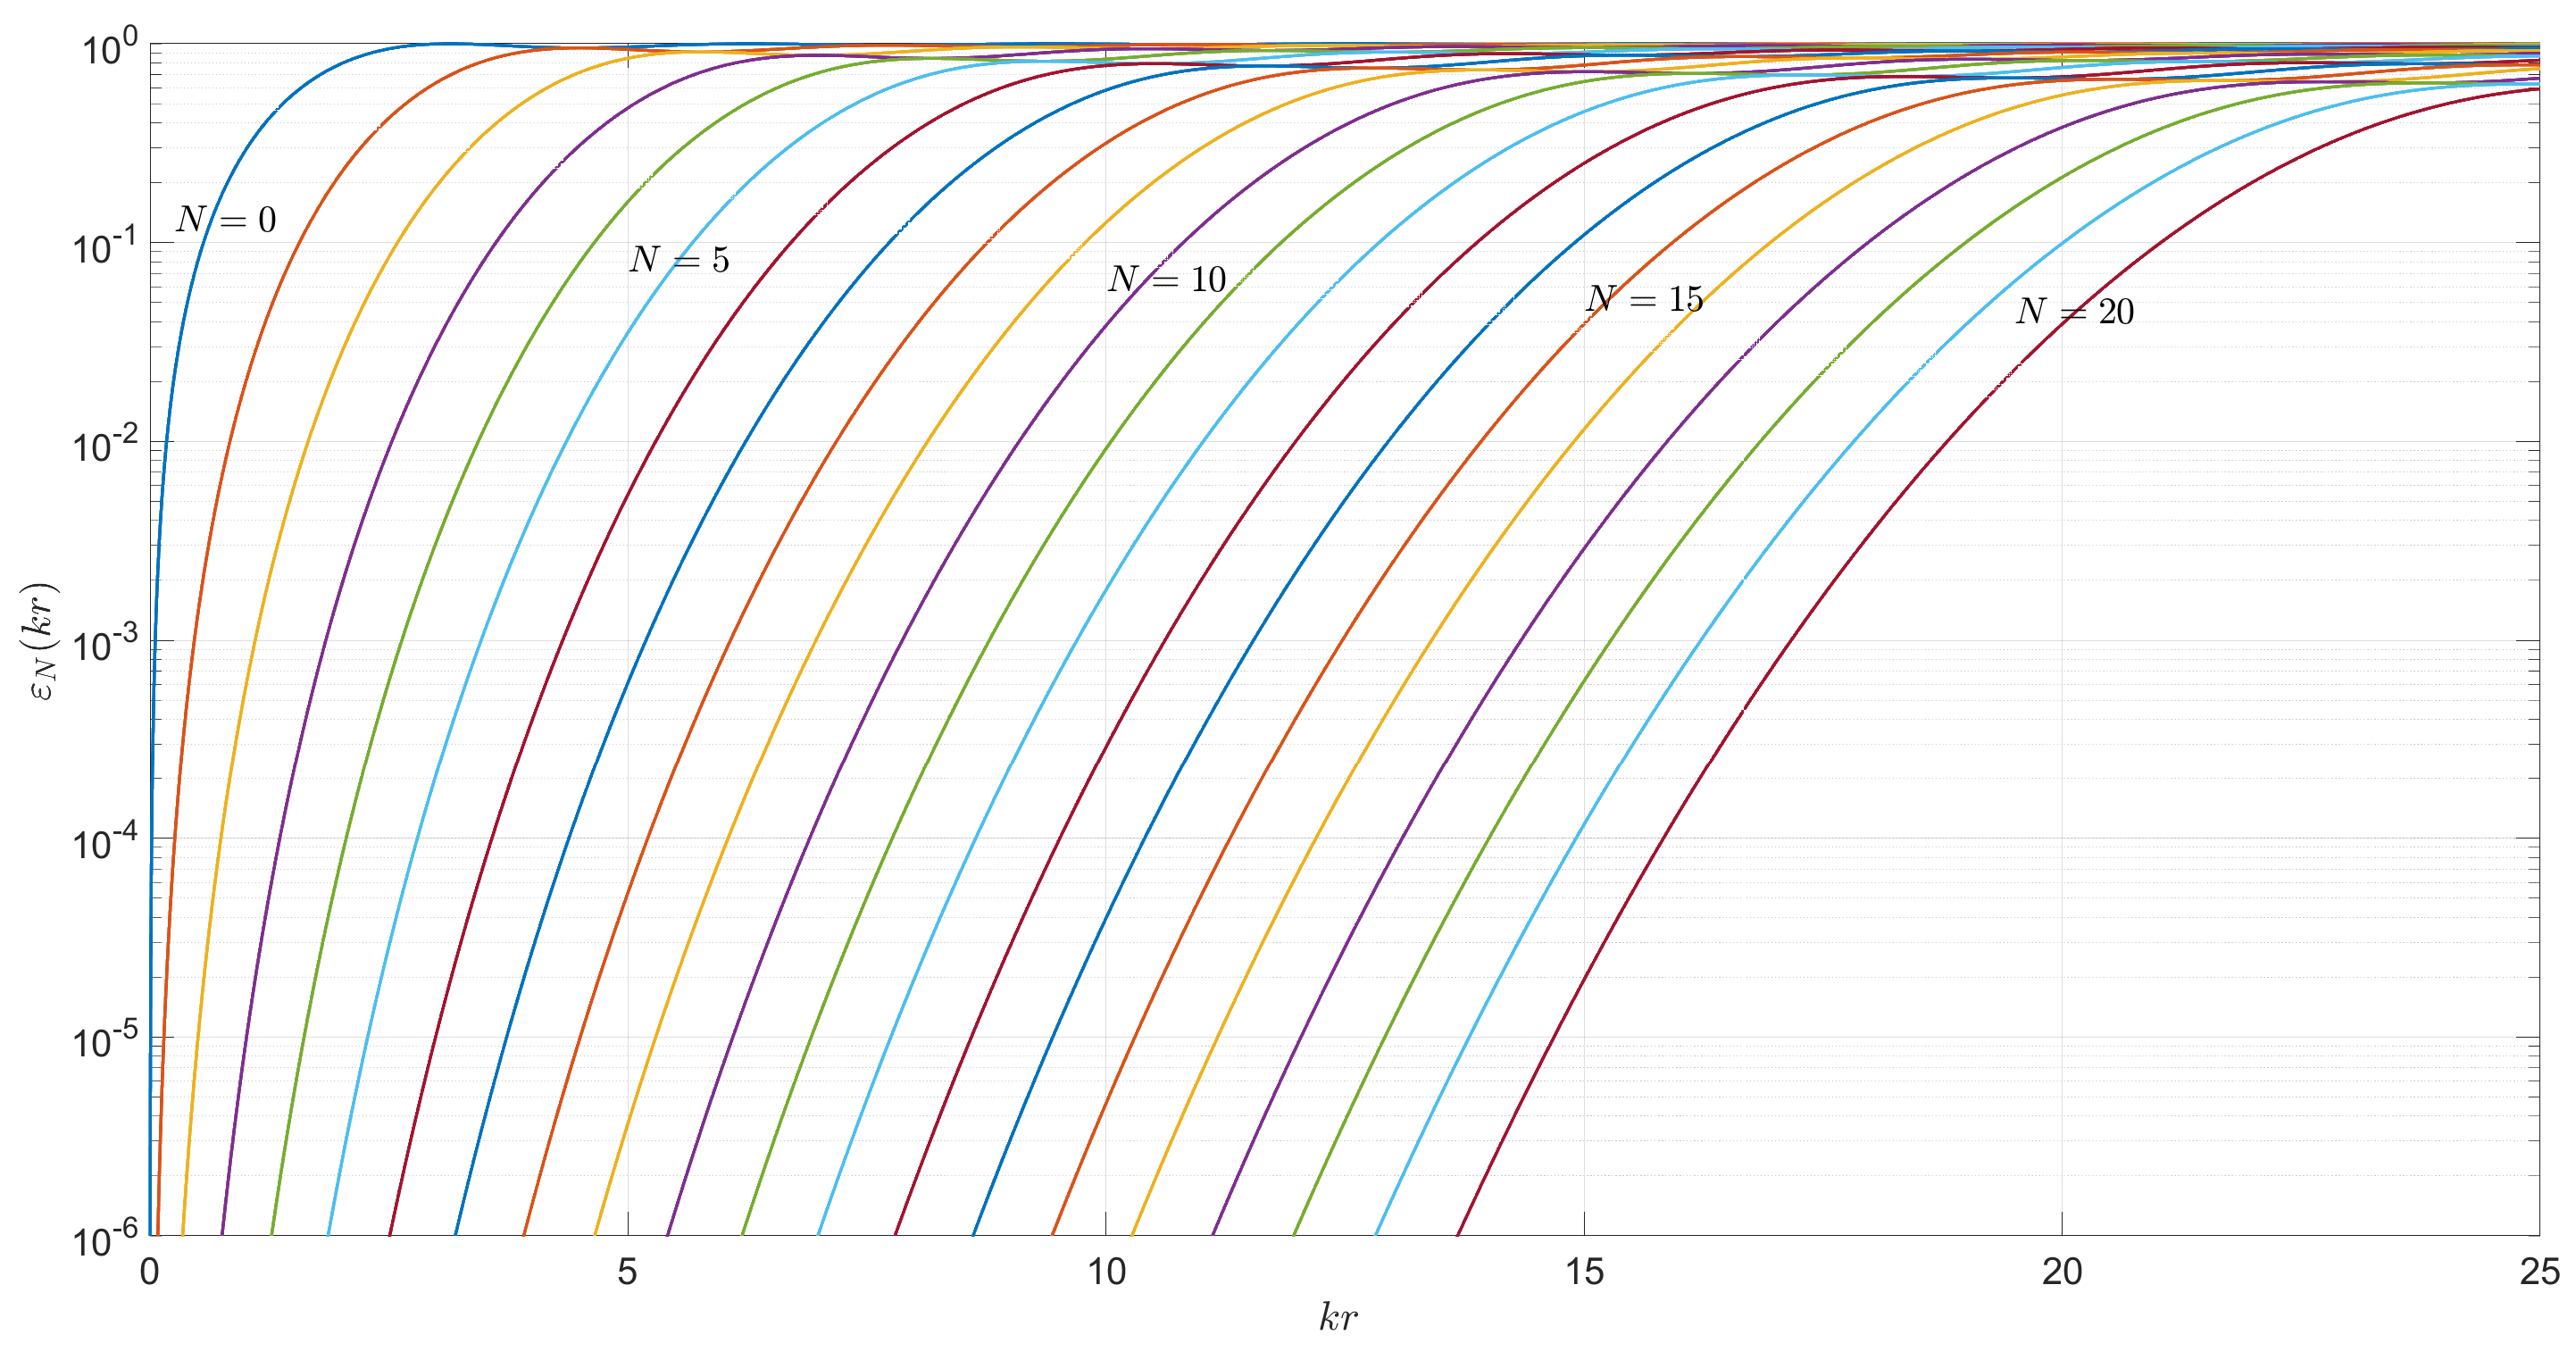
\includegraphics[width=0.9\textwidth]{figure/chapter2/N_kR.eps}
\caption{ 不同阶数~$N$~时归一化截断误差~$\varepsilon _N(kr)$~与~$kr$~的之间的关系}\label{Fig:N_kR}
\label{Fig:N_kR}
\end{figure}

在实际应用中,对于给定的频率~$k$、区域半径~$r$~以及可接受的误差,可以从图~\ref{Fig:N_kR}~查询所需要的分解阶次~$N$。以~$4\%$~的误差为例\tcite{Ward2001Reproduction}(对于大多数实际应用已经足够),可以看出频率~$k$、半径~$r$~和最低截断阶次~$N_{0}$~之间存在关系:
\begin{equation}\label{eq.krN}
   N_0=\lceil kr_0 \rceil,
\end{equation}
式中~$\lceil \cdot \rceil$~表示向上取整。

在半径小于~$r_0$~的重建区域内,重建声场可近似表示原始声场;在半径大于~$r_0$~的重建区域内,重建声场与原始声场差异较大,重建效果不准确。


\subsection{Ambisonics~解码}\label{Ambisonics_decoding}

Ambisonics~解码过程需要满足平面波声场的假设条件,扬声器均匀分布在球上,且只辐射平面波,实现扬声器阵列中心处的声场重建。
采用扬声器阵列重现声场的关键在于求取各个扬声器的激励信号,求解方法为使扬声器阵列产生的声场与原始平面波声场相匹配。原则上,通过使用~Ambisonics~分量信号的线性组合来导出扬声器信号,其中每个信号取决于扬声器相对于重建声场中心的实际位置。接下来从理论上对扬声器激励信号的求解过程进行推导。

由于假设扬声器只辐射平面波,参考式~\eqref{eq.coeS_planewave_N},使用~$L$~个位于~$(\theta_{l},\phi_{l})$~的扬声器进行声场重建时,所产生的线性叠加声场表示为:
\begin{equation}\label{eq.loudspeaker_array}
   \hat{P}(r,\theta,\phi,f)= \sum_{l=1}^{L} w_{l} \sum _{n=0}^{N} \sum _{m=-n}^n 4\pi i^{n} j_n(kr)\left[ Y_n ^m(\theta_{l},\phi_{l}) \right] ^{*} Y_n ^m(\theta,\phi),
\end{equation}
其中,$w_{l}$~为第~$l$~个扬声器的激励信号。

结合式~\eqref{eq.coeS_planewave_N}~和式~\eqref{eq.loudspeaker_array},建立扬声器阵列产生的总声场与原始平面波声场之间的等式:
\begin{equation}\label{eq.mode_matching}
   \sum_{l=1}^{L} w_{l} \left[ Y_n ^m(\theta_{l},\phi_{l}) \right] ^{*}  = \left[ Y_n ^m(\theta_{s},\phi_{s})\right] ^{*}.
\end{equation}

将式~\eqref{eq.mode_matching}~写为矩阵形式:
\begin{equation}\label{eq.min_error_odd_matrix}
\bm{\Psi w}=\bm{d},
\end{equation}
其中,$\mathbf{\Psi}$~是大小为~$(N+1)^2\times L$~的矩阵,其第~$v$~行~$l$~列元素~$\Psi_{v,l} = Y_{n}^{m}(\theta_{l},\phi_{l})$,其中~$v=n^2+n+m+1$,$\bm{w}$~是包含扬声器激励信号的矢量,
\begin{equation}\label{eq.matrix_a}
\bm{w} = [w_{1}~,~w_{2}~,~\cdots~,~w_{L}]^{T},
\end{equation}
\begin{equation}\label{eq.matrix_d}
\mathbf{d} = [Y_{0}^{0}(\theta_{s}~,~\phi_{s})~,\cdots,~Y_{n}^{m}(\theta_{s},\phi_{s})~,~\cdots~,~Y_{N}^{N}(\theta_{s},\phi_{s})]^{T}.
\end{equation}

由于扬声器阵列的配置方式是一定的,因此只有~$\bm{w}$~是未知量。根据球谐系数的数量~$(N+1)^2$~和扬声器的数量~$L$~之间的大小关系,对~$\bm{w}$~的求解分情况讨论~\tcite{Ward2001Reproduction,bookMatrix}:
\begin{compactitem}
\item 当~$L>(N+1)^2$~时,矩阵~$\bm{\Psi}$~是一个欠定矩阵,式~\eqref{eq.min_error_odd_matrix}~可能没有解,也可能有无穷多个解。$\bm{w}$~通常可以通过最小二乘问题求解:
    \begin{equation}
    \mathop{\min}_{\bm{w}} \| \bm{w} \|^{2}~~~\text{subject to}~~\bm{\Psi w = d}
    \end{equation}
    其中,$\| \cdot \|$~表示向量的~2~范数。
\item 当~$L=(N+1)^2$~时,矩阵~$\mathbf{\Psi}$~是一个非奇异方阵,式~\eqref{eq.min_error_odd_matrix}~有唯一解,采用矩阵求逆的方法求解~$\bm{w}$~:
    \begin{equation}
    \bm{w}_{\text{opt}} = \bm{\Psi}^{-1}\bm{d}.
    \end{equation}
\item 当~$L<(N+1)^2$~时,矩阵~$\bm{\Psi}$~是一个超定矩阵,式~\eqref{eq.min_error_odd_matrix}~没有准确解。$\bm{w}$~通常可以通过下式求解:
    \begin{equation}
    \mathop{\min}_{\bm{w}} \| \bm{\Psi w- d} \|^{2}
    \end{equation}

\end{compactitem}

并且在实际系统中,精确再现原始声场所需的扬声器数量为~$L\geq(N+1)^2$,即保证扬声器的数目大于需要约束的模态数~\tcite{Ward2001Reproduction}。

对于一阶~Ambisonics~来说,只包含零阶分量~$W$~和一阶分量~$X$~、$Y$~、$Z$,其扬声器激励信号也可以通过以下方式进行求解。
假设扬声器阵列均匀布放,且扬声器数目~$L\geq4$~,则扬声器激励信号为:
\begin{equation}
w_{l} = \bar{w}_{l}W + \bar{x}_{l}X + \bar{y}_{l}Y + \bar{z}_{l}Z,
\end{equation}
其中,
\begin{equation}
\begin{split}
\bar{w}_{l} & = \sqrt{2}/L \\
\bar{x}_{l} & = 3\cos\phi_{l}\cos\theta_{l}/L \\
\bar{y}_{l} & = 3\sin\phi_{l}\cos\theta_{l}/L \\
\bar{z}_{l} & = 3\sin\theta_{l}/L
\end{split}
\end{equation}



\subsection{虚拟扬声器方法}

在多通路环绕声系统中,为了产生空间中某一方向的虚拟源,并不一定需要在此方向布放一个扬声器,而是可以在空间中适当地布置若干个扬声器,通过调整各个扬声器的激励信号来产生不同方位的虚拟源。借鉴多通路环绕声系统,在双耳合成过程中,可以分别合成多个不同方位的虚拟扬声器,通过改变各个虚拟扬声器的激励信号,即可模拟出多通道声重放中不同虚拟源产生的双耳声信号。虽然这种双耳信号可能只是理想情况的低阶近似,但利用多声源综合定位的心理学原理,可在耳机重放中得到相应空间虚拟源的听觉感知~\tcite{jot1998approaches}\tcite{jot1999comparative}。这就是双耳合成中虚拟扬声器(virtual loudspeaker)方法的基本思路。 % 本段来源于《空间声原理》

由~\ref{Ambisonics_decoding}~节可以得到声场重现所需的虚拟扬声器摆放方式和对应的扬声器激励信号,为了让~Ambisonics~系统可以用于耳机实现,我们需要对虚拟扬声器信号加以~HRTF~渲染,该方法可以消除听音空间对扬声器回放产生的影响。

假设整个空间中有~$L$~个虚拟声源(虚拟扬声器),其位置为~$(\theta_{l},\phi_{l})$,激励信号为~$w_{l}(f)$,双耳接收到的信号是多个声源共同作用的结果:
\begin{equation}\label{eq.loudspeaker_to_headphone}
\begin{split}
B_{\text{L}}(f) = \sum_{l=1}^{L}H_{\text{L}}(\theta_{l},\phi_{l},f)w_{l}(f)\\
B_{\text{R}}(f) = \sum_{n=l}^{L}H_{\text{R}}(\theta_{l},\phi_{l},f)w_{l}(f),
\end{split}
\end{equation}
其中,$H_{\text{L}}(\theta_{l},\phi_{l},f)$~和~$H_{\text{R}}(\theta_{l},\phi_{l},f)$
是声源位于~$(\theta_{l},\phi_{l})$~处的左、右耳~HRTF~数据。
最后对~$B_{\text{L}}(f)$~和~$B_{\text{R}}(f)$~求反傅里叶变换即可得到时域双耳信号。

但是基于~Ambisonics~的虚拟扬声器方法会带来一些问题:一是不同的虚拟扬声器数目和位置会对所获取的双耳信号带来影响,二是扬声器所在位置的声像会不可避免地被加重。并且当扬声器所处方位在现有的~HRTF~数据库中没有对应的数据,此时需要对原始~HRTF~进行插值。

\section{基于球谐分解的双耳渲染算法}\label{sec.SHdecomposition}

近年来,基于球谐分解的双耳渲染算法受到人们的广泛关注。其核心思想是不仅对声场进行球谐分解,同时对~HRTF~进行球谐分解,直接在球谐域上进行渲染。可以避免了虚拟扬声器引入对双耳信号带来的影响。

对声场使用球谐函数进行表示:
\begin{equation}
S(r,\theta,\phi,f) = \sum_{n=0}^{N_{s}}\sum_{m=-n}^{n} S_n^m(r,f)Y_{n}^{m}(\theta,\phi),
\end{equation}
其中,$S_n^m(r,f)$~是声学场景的球谐系数,无需声源信号和方位的先验信息。$N_{s}$~为声场的球谐分解阶次,由录制设备决定。

HRTF~一般在一个固定的球面上进行多点采样,当球面半径大于~1~米时,可以认为是远场~HRTF~,可以使用球谐函数进行分解:
\begin{equation}\label{HRTF_decomposition}
\begin{split}
H_{\text{L}}(\theta,\phi,f) & = \sum_{n=0}^{N_{h}}\sum_{m=-n}^{n} \beta_{nm}^{\text{L}}(f)Y_{n}^{m}(\theta,\phi) \\
H_{\text{R}}(\theta,\phi,f) & = \sum_{n=0}^{N_{h}}\sum_{m=-n}^{n} \beta_{nm}^{\text{R}}(f)Y_{n}^{m}(\theta,\phi),
\end{split}
\end{equation}
其中,$N_{h}$~是~HRTF~进行球谐分解的阶数。

由于声源可能具有一定体积,例如面源、体源,并且房间混响会产生反射,因此假设声场中声源是连续分布的,则左耳的信号可以表示为~\tcite{Benesty2008Microphone}\tcite{2013Study}\tcite{2016Fundamentals}:
\begin{align}
B_{\text{L}}(f) &= \int_{0}^{2\pi}\int _{0}^{\pi}S(r,\theta,\phi,f)\left[H_{\text{L}}(\theta,\phi,f)\right]^{*}\sin \theta d\theta d\phi \nonumber \\
&= \int_{0}^{2\pi}\int _{0}^{\pi} \sum_{n=0}^{N_{s}}\sum_{m=-n}^{n} S_n^m(r,f)Y_{n}^{m}(\theta,\phi) \left[  \sum_{n'=0}^{N_{h}}\sum_{m'=-n'}^{n'} \beta_{n'm'}^{\text{L}}(f)Y_{n'}^{m'}(\theta,\phi)\right]^{*}
\sin\theta d\theta d\phi \nonumber \\
&=\sum_{n=0}^{N_{s}}\sum_{m=-n}^{n} \sum_{n'=0}^{N_{h}}\sum_{m'=-n'}^{n'} S_n^m(r,f)\left[\beta_{n'm'}^{\text{L}}(f)\right]^{*}
\int_{0}^{2\pi}\int _{0}^{\pi} Y_{n}^{m}(\theta,\phi)\left[Y_{n'}^{m'}(\theta,\phi)\right]^{*}\sin\theta d\theta d\phi \nonumber \\
&= \sum_{n=0}^{N}\sum_{m=-n}^{n} S_n^m(r,f)\left[\beta_{nm}^{\text{L}}(f)\right]^{*},
\label{eq.BL}
\end{align}
其中,$N=\min \left\{ N_{s},N_{h} \right\}$,最后一个等式的推导借助了球谐函数的正交性,如式~\eqref{eq.orth}~所示。

同理,右耳信号可以表示为:
\begin{equation}
B_{\text{R}}(f) = \sum_{n=0}^{N}\sum_{m=-n}^{n} S_n^m(r,f) \left[ \beta_{nm}^{\text{R}}(f)\right]^{*}
\label{eq.BR}
\end{equation}


由~$N=\min \left\{ N_{s},N_{h} \right\}$~可知,在球谐域上进行双耳渲染时的球谐阶次由声场和~HRTF~进行球谐分解的阶次共同决定。HRTF~数据库的球面采样点较为密集,可以实现高阶球谐系数的获取,并且研究表明,要想对高达~15~kHz~的~HRTF~进行精确的物理表征,大约需要~$N_{h}= 34$~的阶次。声场方面,要想准确获取~$N$~阶声场,至少需要~$(N+1)^2$~个采样点,其详细推导见第~\ref{section_microphone_array_coe}~节,而实际系统中,对~$N_{h}=34$~对应的~1225~个通道的采集、传输和处理很难实现,一般来说录制设备的通道数较少,所能准确获取的声场系数的阶次较低,基本满足~$N_{s}<5$~\tcite{2018Binaural}。
二者之间的阶次存在不匹配问题,HRTF~虽然可以获取高阶球谐分量,但也只能使用低阶进行表示。HRTF~的直接低阶截断会导致高频能量损失,带来一定的误差。除此之外,还存在其他问题,例如录音设备的尺寸小于人头尺寸,录音设备的采样率与~HRTF~数据库采样率不一致等。
这些不匹配问题将会导致所获取的双耳信号的空间分辨率受限、定位线索(双耳时间差~ITD、双耳声级差~ILD)的损伤、空间感的下降等,直接影响声源方位的感知、外化~(externalization)、感知声源宽度和音色等~\tcite{sheaffer2014rendering}\tcite{2013Spatial}\tcite{2015Efficient}\tcite{2017equalization}。


本文主要针对以上问题,对基于球谐分解的双耳渲染算法进行研究,对头相关传递函数~HRTF~的预处理加以研究,并且从另外一个方面~——~声场出发,提出改进方法。

\newpage
\section{本章小节}
本章主要介绍了几种常见的双耳渲染技术及其原理。 首先对基于~HRIR~和~BRIR~的虚拟听觉的方法进行了简单介绍,其中头相关传递函数~HRTF~是所有双耳渲染算法中的核心数据。接下来对基于~Ambisonics~的虚拟扬声器方法进行了详细推导,其核心思想是对声场的球谐分解,再利用各阶谐波分量求解重建声场所需的扬声器设置和对应的激励信号,最后结合虚拟扬声器获取双耳信号,其中对声场进行正交球谐分解是本文的重要理论基础。最后对基于球谐分解的双耳渲染技术进行了介绍和理论推导,并对其所存在的问题进行了简单描述,本文将在此算法框架下进行,针对其所存在的问题,提出改进算法。